% Thesis chapter: the simulated crane testbed (Isaac Lab).
% Standalone chapter file; \input or \include from the thesis root.
% Synthesizes the physics-tuning material of the original Isaac Sim environment
% (still inherited by the current assets) with the Isaac Lab environment,
% FSM controller, and task formulation.

\chapter{A Simulated Crane Testbed for Pile-Scale Clearing}
\label{ch:sim_env}

All learning in this thesis happens in simulation. This chapter describes the
simulated testbed: the crane model and its passively suspended grapple, the
physics modeling required to keep hundreds of contacting logs stable and
realistic, the fixed grasp-cycle controller, and the decision-level task
formulation that every method in the thesis shares. The environment is
implemented in Isaac Lab~\cite{mittal2025isaaclab} on PhysX GPU dynamics and
runs tens of environments in parallel on a single laptop GPU
(Figure~\ref{fig:sim_env_scene}), which is what
makes both large-scale demonstration collection and on-policy reinforcement
learning practical.

\section{Crane Model}

The simulated machine reproduces the FPInnovations log-loader testbed: a
trailer-mounted hydraulic crane with a grapple suspended from a passive
articulated hanger (Figure~\ref{fig:sim_crane_links}). The arm has four
actuated joints, a slewing base-mast joint, boom and stick revolute joints,
and a prismatic telescope, followed by a two-link passive chain that
suspends the grapple from the telescope tip. The passive joints are unactuated revolute
joints, modeling the gravity-driven hanging behavior of a real grapple
attachment: the grapple body hangs roughly 0.4~m below the commanded telescope
tip and swings like a pendulum during arm motion. Below the chain, a yaw joint
actively rotates the grapple about the vertical axis and two tong joints open
and close the jaws. Link masses and joint limits are listed in
Table~\ref{tab:sim_params}; they follow the testbed's URDF description.

\begin{figure}[t]
\centering

\includegraphics[width=\linewidth]{crane_links.pdf}
\caption{The simulated crane and its links. The four actuated arm joints
(slew at the crane base, boom, stick, telescope) carry a two-link passive
chain, below which the grapple yaw joint and the tongs act. Inset: the
passive chain pivots freely in two axes, so the grapple hangs under gravity
and swings during arm motion, while the yaw joint sets the grapple heading
$\psi$. The two stereo cameras are shown at the mounts they occupy on the
physical machine (Chapter~\ref{ch:sim2real}).}
\label{fig:sim_crane_links}
\end{figure}

\begin{figure}[t]
\centering

\includegraphics[width=\linewidth]{crane_env_basemast.pdf}
\caption{The simulated testbed. Left: parallel environment instances, each
with an independently randomized pile, stepped together on the GPU. Right: a
single environment with the frames the task is expressed in. The policy
observes a point cloud and selects a grasp target inside the rack-aligned
action volume (green), and a fixed state machine executes the cycle.}
\label{fig:sim_env_scene}
\end{figure}

The passive chain deserves emphasis because it shapes both control and
evaluation. Because the grapple is not rigidly attached, every commanded
motion excites swing that must decay before a grasp can be executed
accurately, and the tilt of the suspended load after lifting is the physical
signal behind the stability metric of Section~\ref{sec:sim_outcome}. The
fidelity of the chain's spring-damper model turned out to matter: the values
used during the early simulation campaigns (stiffness 300, damping 500 in the
chain joints) suppress swing more strongly than the real, freely pivoting
hanger, with consequences for stability measurements that are taken up in
Section~\ref{sec:sim_study_stability} and Chapter~\ref{ch:sim2real}. The
corrected configuration frees the pivots (zero stiffness with light damping).

\section{Physics Modeling and Tuning}

Simulating a dense pile is a different regime from typical robotics scenes:
several hundred rigid bodies rest in persistent frictional contact, and the
grapple deliberately drives into the contact network. Default physics
settings failed outright, with logs ricocheting on spawn, chain-reaction
pile explosions on grapple contact, and scene crashes beyond roughly 300
bodies. The configuration below was reached by systematic tuning on the
original Isaac Sim implementation of the scene and is inherited by the Isaac
Lab environment, which reuses the same assets and physics parameters.

\subsection{Log assets from field measurements}

Log geometry and mass follow direct measurements of ten logs at the
FPInnovations testbed (Table~\ref{tab:log_measurements}). The simulation log
is a cylinder of diameter 0.113~m and length 2.45~m with a mass of 15~kg,
matching the measured averages. Logs are instanced from a single prototype
asset~\cite{blender, nvidia_instancing}, which keeps memory usage flat in the
number of logs, guarantees identical physical properties across instances,
and lets material or collision changes be applied globally during tuning.

\begin{table}[t]
\centering
\caption{Field measurements of the testbed logs (two end diameters D1, D2).
The simulated log uses the rounded averages: diameter 0.113~m, length 2.45~m,
mass 15~kg.}
\label{tab:log_measurements}
\begin{tabular}{ccccc}
\hline
\textbf{Log} & \textbf{D1 (mm)} & \textbf{D2 (mm)} & \textbf{Length (mm)} & \textbf{Mass (kg)} \\
\hline
1 & 101 & 86 & 2480 & 12.2 \\
2 & 104 & 123 & 2390 & 14.2 \\
3 & 72 & 113 & 2600 & 11.8 \\
4 & 120 & 132 & 2480 & 17.4 \\
5 & 121 & 94 & 2560 & 15.6 \\
6 & 124 & 142 & 2450 & 18.1 \\
7 & 110 & 129 & 2550 & 18.0 \\
8 & 89 & 110 & 2550 & 9.7 \\
9 & 126 & 110 & 2290 & 15.8 \\
10 & 136 & 114 & 2180 & 15.6 \\
\hline
Mean & 110.3 & 115.3 & 2453 & 14.8 \\
\hline
\end{tabular}
\end{table}

Contact material properties use published oak-on-oak friction coefficients
($\mu_s = 0.62$, $\mu_k = 0.48$)~\cite{avallone2006marks} with near-zero
restitution (0.05) so that impacts dissipate energy. Friction combines by
maximum and restitution by minimum across contact pairs~\cite{nvidia_combine},
the conservative choices for stability. With these values, spawned logs settle
into piles with realistic angles of repose, grasped bundles cohere through
friction during transport, and released logs come to rest within one to two
seconds without bouncing.

\subsection{Collision geometry and detection}

Collision representations are chosen per component~\cite{nvidia_colliders}:
convex hulls for logs (an efficient 32-vertex cylinder approximation), convex
decomposition for the rack so its concave cradle actually contains logs, and
signed-distance-field (SDF) meshes for the grapple tongs, whose curved,
interlocking geometry needs smooth contact normals for multi-log grasps to
close reliably. Continuous collision detection is enabled for logs and
grapple parts~\cite{nvidia_ccd}, eliminating tunneling during pile settling,
fast approaches, and log release.

\subsection{Solver}

The constraint solver choice proved decisive. The default temporal
Gauss-Seidel (TGS) solver became less stable as iterations increased: its
aggressive convergence injects energy when resolving the deep
interpenetrations that arise inside dense piles, producing explosive
collapses. The projected Gauss-Seidel (PGS) solver, with high position and
velocity iteration counts, resolves the same contact networks
conservatively~\cite{nvidia_solver} and is used throughout. Physics runs at
120~Hz with a control decimation of two (60~Hz control).

\subsection{Actuation and pile initialization}

Actuated joints use implicit PhysX PD drives ($k_p = 10^6$,
$k_d = 10^5$)~\cite{nvidia_joints}, with torque limits sized from the loads of
multi-log lifts; the grapple yaw joint and tongs use lower gains, with the
tongs driven by a saturated PD velocity law with discrete stepping to avoid
abrupt contact forces. Piles are initialized by spawning logs in a layered
grid above the rack with small random perturbations, then simulating until
maximum linear and angular velocities fall below thresholds; the settled
configuration becomes the episode's initial state. Randomization over log
count, grid dimensions, spacing, layer offsets, and per-log jitter (and, in
later data-collection recipes, profiled mound shapes) generates pile
diversity across episodes.

\begin{table}[t]
\centering
\caption{Principal simulation and controller parameters. Actuator gains are
implicit PhysX joint-drive values. The passive-chain values in parentheses are
the corrected free-pivot configuration adopted after hardware comparison
(Section~\ref{sec:sim_study_stability}).}
\label{tab:sim_params}
\small
\begin{tabular}{lr}
\hline
\textit{Simulation} & \\
Physics timestep & $1/120$ s \\
Control decimation & $2\times$ (60 Hz) \\
\hline
\textit{Crane link masses} & \\
Mast / main boom / stick & 290 / 172 / 70 kg \\
Telescope / passive chain links & 25 / 9 kg \\
\hline
\textit{Joint limits} & \\
Base-mast (revolute) & $\pm 100^{\circ}$ \\
Boom (revolute) & $-22^{\circ}$ to $+75^{\circ}$ \\
Stick (revolute) & $-177^{\circ}$ to $+2^{\circ}$ \\
Telescope (prismatic) & 0.13--1.80 m \\
Grapple yaw (revolute) & $\pm 180^{\circ}$ \\
\hline
\textit{Actuator gains} ($k_p$ / $k_d$) & \\
Main arm joints & $10^{6}$ / $10^{5}$ \\
Passive chain & 300 / 500 \; (corrected: 0 / 100) \\
Grapple yaw & $5\times 10^{4}$ / $2\times 10^{4}$ \\
Grapple tongs & 0 / 500 \\
\hline
\textit{Log properties} & \\
Diameter / length & 0.113 / 2.45 m \\
Mass & 15 kg \\
Friction $\mu_s$ / $\mu_k$ & 0.62 / 0.48 \\
Restitution & 0.05 \\
Contact / rest offset & 0.02 / 0.0 m \\
\hline
\textit{FSM parameters} & \\
Hover clearance & 2.5 m \\
Position tolerance (chain top / grapple) & 0.10 / 0.25 m \\
Dwell count & 30 steps \\
Phase timeout & 100 steps \\
\hline
\end{tabular}
\end{table}

\section{The Grasp-Cycle State Machine}
\label{sec:sim_fsm}

All methods in this thesis, heuristic and learned alike, share one fixed
execution controller: a finite state machine (FSM) that turns a commanded
grasp target $(x, y, z, \psi)$ into a complete grasp cycle. The arm is driven
by Isaac Lab's damped-least-squares differential inverse-kinematics
controller in task space; the grapple yaw joint is position-controlled
independently. Because the IK target is the top of the passive chain while
the grasp happens at the grapple body hanging below it, targets are specified
for the grapple and offset vertically to the IK link, and each phase uses a
two-stage convergence check: the IK link must reach its target within
0.10~m, then the grapple body must settle within 0.25~m, both holding for 30
consecutive steps so that pendulum oscillation has died out before the cycle
proceeds. A per-phase timeout forces advancement if convergence is not
reached, preventing stalls on difficult configurations.

The cycle has five phases: \texttt{HOVER} moves the grapple above the target
with 2.5~m clearance; \texttt{ALIGN} rotates the grapple to the commanded
yaw; \texttt{DESCEND} lowers it at reduced speed to limit pile disturbance;
\texttt{CLOSE} shuts the jaws with discrete velocity stepping; and
\texttt{LIFT} raises the load back to hover height and holds it while the
grasp outcome is evaluated. In the grasp-and-remove configuration used for
the simulation study of Chapter~\ref{ch:sim_study}, grasped logs are then
removed from the scene and the cycle repeats; the environment also supports
full transport-and-deposit cycles, which are used in the deployment-aligned
configuration of Chapter~\ref{ch:sim2real}.
Algorithm~\ref{alg:fsm} states the cycle; parameter values are in
Table~\ref{tab:sim_params}.

\begin{algorithm}[t]
\caption{Grasp-cycle state machine, shared by every method in this thesis}
\label{alg:fsm}
\begin{algorithmic}
\algin{Grasp target $\mathbf{g} = (x, y, z, \psi)$; hover clearance $h$;
tolerances $\epsilon_{\mathrm{ik}}$ (chain top) and $\epsilon_{\mathrm{gr}}$
(grapple body); dwell count $D$; per-phase timeout $T_{\max}$.}
\algout{Cycle outcome $(n, \alpha, \varsigma)$ of Section~\ref{sec:sim_outcome}.}

\Function{Settle}{target $\mathbf{p}$}
  \Comment{two-stage convergence, run every control step}
  \State Command the chain-top IK link to $\mathbf{p}$ offset vertically for the hanging grapple
  \State Wait until $\lVert \mathbf{p}_{\mathrm{ik}} - \mathbf{p} \rVert < \epsilon_{\mathrm{ik}}$,
         \textbf{then} until $\lVert \mathbf{p}_{\mathrm{grapple}} - \mathbf{p} \rVert < \epsilon_{\mathrm{gr}}$
  \State Require both to hold for $D$ consecutive steps
  \Comment{lets swing decay first}
  \State Advance regardless after $T_{\max}$ steps
  \Comment{timeout prevents stalls}
\EndFunction

\algstage{1.\;\texttt{HOVER}}
\State \Call{Settle}{$(x, y, z + h)$}

\algstage{2.\;\texttt{ALIGN}}
\State Drive the grapple yaw joint to $\psi$ and hold position

\algstage{3.\;\texttt{DESCEND}}
\State \Call{Settle}{$(x, y, z)$} at reduced command scale
\Comment{limits pile disturbance}

\algstage{4.\;\texttt{CLOSE}}
\State Close the tongs under a saturated velocity law with discrete stepping

\algstage{5.\;\texttt{LIFT}}
\State Raise to $(x, y, z + h)$ and hold while the load settles
\State Evaluate the outcome: throughput $n$, alignment $\alpha$, stability $\varsigma$
\State Remove grasped logs (grasp-and-remove) or continue to transport and release
\State \Return $(n, \alpha, \varsigma)$
\end{algorithmic}
\end{algorithm}

\section{Task Formulation}
\label{sec:sim_task}

\subsection{A decision-level MDP}

The learning problem is formulated at the level of grasp decisions rather
than joint commands: one environment step is one complete grasp cycle, an
abstraction in the spirit of temporally extended
actions~\cite{sutton1999between}. The state is the pile configuration,
observed either as a point cloud or, for privileged baselines, as log poses;
the action is the grasp target; the transition is whatever the physics and
the FSM produce; and one scalar reward summarizes the cycle's outcome. An
episode ends when the rack is empty or after a fixed budget of $H = 30$ grasp
attempts, chosen with roughly 50\% margin over what the scripted expert needs
to clear a 200-log pile. Horizons of tens of decisions, rather than
thousands of control steps, are what make on-policy fine-tuning with a
privileged critic practical in Chapters~\ref{ch:sim_study} and \ref{ch:bcrl}.

\subsection{Observations}
\label{sec:sim_obs}

The policy observes a point cloud derived from a simulated depth camera
above the rack, with pinhole intrinsics matching the Stereolabs ZED~X used on
the physical testbed. Valid depth pixels are back-projected through the
intrinsics, transformed into the crane base frame using the known camera
extrinsics, cropped to a box around the rack, and downsampled with farthest
point sampling (FPS) to a fixed budget of $N$ points (1024 in the simulation
study; 2048 in the widened deployment pipeline of
Chapter~\ref{ch:bc_policies}); short clouds are zero-padded.
Algorithm~\ref{alg:obs_pipeline} states the procedure, and
Figure~\ref{fig:sim_pcd_pipeline} shows it applied to one decision.
Critically, no segmentation is applied at any stage: the cloud contains every
surface the camera sees, including rack structure and ground, and the
network must learn what is graspable. As a privileged ablation, some
baselines instead observe the top-$K$ log poses ($K = 32$), height-sorted, as
a compact $4K$-dimensional vector $\xi_t$; the comparison isolates the cost of
perception from the learning algorithm.

The same procedure runs at deployment, with the simulated camera replaced by
the physical one and the known extrinsics replaced by the calibrated mount of
Section~\ref{sec:s2r_camcalib}. Keeping it operation for operation identical
is a hard requirement rather than a convenience: any step that differs
between the two is a distribution shift the policy pays for directly, so
Algorithm~\ref{alg:obs_pipeline} is the single definition referenced by both
the training pipelines of Chapter~\ref{ch:bc_policies} and the deployed node
of Section~\ref{sec:s2r_deploy}.

\begin{algorithm}[t]
\caption{Observation pipeline (identical in simulation and at deployment)}
\label{alg:obs_pipeline}
\begin{algorithmic}
\algin{Depth image $Z$ with pinhole intrinsics $K_{\mathrm{cam}}$; extrinsic
$T_{\mathrm{base} \leftarrow \mathrm{cam}}$; action box
$[b^{\min}, b^{\max}]$; crop margin $m$; point budget $N$.}
\algout{Observation cloud $P \in \mathbb{R}^{N \times 3}$ in the crane base
frame, with a padding mask.}

\algstage{1.\;Back-projection}
\State Discard invalid depth pixels; back-project the rest through
$K_{\mathrm{cam}}$ to camera-frame points $P_{\mathrm{raw}}$.

\algstage{2.\;Base-frame transform}
\State $P \gets T_{\mathrm{base} \leftarrow \mathrm{cam}}\, P_{\mathrm{raw}}$
\Comment{known in simulation, calibrated on the crane}

\algstage{3.\;Crop}
\State $P \gets \{\, p \in P \;:\; b^{\min} - m \preceq p \preceq b^{\max} + m \,\}$
\Comment{no segmentation; structure and ground are kept}

\algstage{4.\;Resample to a fixed budget}
\If{$|P| > N$}
  \State $P \gets \mathrm{FPS}_N(P)$ \Comment{farthest point sampling}
\Else
  \State Zero-pad $P$ to $N$ rows and mark the padded slots
\EndIf
\State \Return $P$ and the padding mask
\end{algorithmic}
\end{algorithm}

\begin{figure}[t]
\centering
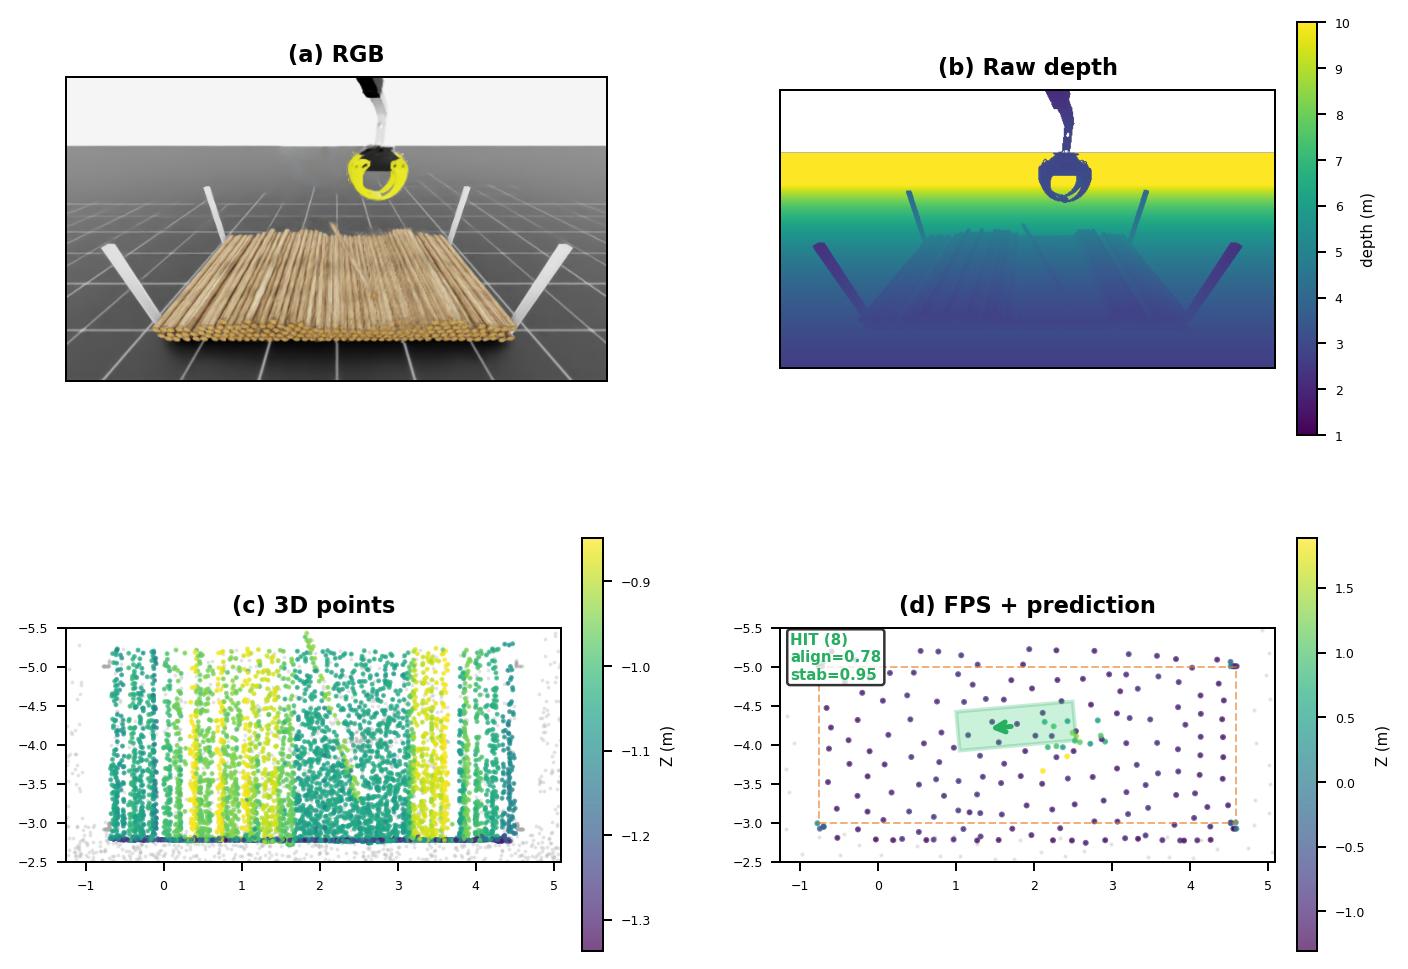
\includegraphics[width=\linewidth]{episode_001_pipeline_quad_single.png}
\caption{Observation pipeline for a single grasp decision. (a)~Camera RGB
view, (b)~raw depth, (c)~3D back-projection in the crane base frame,
(d)~FPS-downsampled point cloud with the policy's grasp target and the
grapple footprint overlaid.}
\label{fig:sim_pcd_pipeline}
\end{figure}

\subsection{Actions}
\label{sec:sim_actions}

A grasp target is the tuple $\mathbf{g} = (x, y, z, \psi)$: the grapple
position in the crane base frame and its yaw about the vertical axis
(Figure~\ref{fig:sim_env_scene}). Learned policies output five unbounded
scalars. The three position components are squashed by $\tanh$ and mapped
linearly into a rack-aligned action box, so every decodable action is a
physically executable target; the box also serves
as the out-of-bounds cull region for logs knocked off the rack. Yaw is
represented by the doubled-angle pair $(\cos 2\psi, \sin 2\psi)$: a
cylindrical log at yaw $\psi$ is identical at $\psi + \pi$, and the
$\pi$-periodic encoding maps the two physically identical grasps to the same
point~\cite{morrison2018closing}, which proves essential for supervised
training (Chapter~\ref{ch:bc_policies}). Expert targets are encoded into the
same pre-squash space, so imitation and reinforcement learning share one
action space.

\subsection{Outcome evaluation}
\label{sec:sim_outcome}

After the lift, the outcome of the cycle is measured by three quantities.
The \emph{throughput} $n$ counts the logs held by the grapple (centers within
a proximity radius). The \emph{alignment}
\begin{equation}
  \alpha_i = \big( \hat{y}_g^{\top} \hat{y}_{\ell_i} \big)^{8}, \qquad
  \alpha = \frac{1}{n} \sum_{i=1}^{n} \alpha_i \in [0, 1],
\end{equation}
scores the angle between the grapple jaw axis $\hat{y}_g$ and each held log's
length axis $\hat{y}_{\ell_i}$; the even exponent absorbs the log's
directional symmetry and the eighth power penalizes moderate misalignment
sharply. The \emph{stability}
\begin{equation}
  \varsigma = \big( \max(0,\; \hat{z}_g^{\top} \hat{z}_w) \big)^{4} \in [0, 1]
  \label{eq:sim_stability}
\end{equation}
scores the levelness of the grapple after lifting, with $\hat{z}_g$ its up
vector and $\hat{z}_w$ the world vertical. Figure~\ref{fig:sim_outcomes}
shows the shaped score curves.

Equation~\eqref{eq:sim_stability} is the \emph{snapshot} form, evaluated from
a single sample at the end of a fixed hold, which is how the metric was
implemented for the campaigns of Chapter~\ref{ch:sim_study}. It was later
replaced by a \emph{windowed} form that mirrors the measurement procedure
running on the physical crane. Writing
$\theta_t = \arccos\big(\max(0,\; \hat{z}_g^{\top} \hat{z}_w)\big)$ for the
tilt sampled at control step $t$ of the post-lift hold,
\begin{equation}
  \varsigma = \big( \cos \bar{\theta} \big)^{4}, \qquad
  \bar{\theta} = \frac{1}{|W|} \sum_{t \in W} \theta_t ,
  \label{eq:sim_stability_windowed}
\end{equation}
where $W$ is the trailing one-second window of the hold, accepted once its
variance stays below $10^{-4}$~rad$^2$ for half a second and otherwise taken
best-effort at a four-second timeout. Averaging the angle before sharpening,
rather than sharpening each sample, keeps the score independent of the
sampling rate and so comparable to the crane's timer-paced measurement; the
clamp inside $\theta_t$ bounds each sample to $[0, \pi/2]$, which is why no
outer clamp is needed in
Equation~\eqref{eq:sim_stability_windowed}. Both forms use the same exponent
and share the interpretation of Figure~\ref{fig:sim_outcomes}; the windowed
form is the one used for the reward and the reported metric in
Chapters~\ref{ch:bc_policies} and~\ref{ch:bcrl}. Which form is in force is
recorded with each result, because the two are not interchangeable: a
snapshot can catch the load at any point of a residual swing, whereas the
windowed value only reports once the swing has actually decayed. That is a
separate issue from the passive-chain modeling error that led one campaign's
stability results to be withdrawn (Section~\ref{sec:sim_study_stability}).

Reported quantities also include the grasp success rate (fraction of cycles
with $n > 0$), the pile clearing rate (fraction of the initial inventory
intentionally grasped and removed), and the fraction of logs knocked out of
bounds.

\begin{figure}[t]
\centering

\includegraphics[width=\linewidth]{outcomes.png}
\caption{Grasp outcome geometry and shaped scores. The per-log misalignment
angle $\theta_{\alpha_i}$ is measured between the grapple closing axis
$\hat{y}_g$ and the log axis $\hat{y}_{\ell_i}$, and the tilt angle
$\theta_\varsigma$ between the grapple vertical $\hat{z}_g$ and the world
vertical. Insets: the shaped alignment score
$\alpha_i = (\cos\theta_{\alpha_i})^8$ and stability score
$\varsigma = (\max(0, \cos\theta_\varsigma))^4$; the sharp exponents
concentrate reward on well-aligned, level grasps.}
\label{fig:sim_outcomes}
\end{figure}

\section{The Privileged Heuristic Expert}
\label{sec:sim_expert}

A scripted expert serves as both a competitive baseline and the
demonstration source for behavior cloning. It has privileged access to the
poses of all active logs and follows a top-of-pile targeting strategy: at
each cycle it selects the log with the highest center, targets that center,
and aligns the grapple yaw with the log's length axis, choosing between the
two symmetric orientations by minimal joint rotation and re-evaluating the
alignment closed-loop during the \texttt{ALIGN} phase
(Algorithm~\ref{alg:expert}). The highest log is
typically the most accessible, with the fewest obstructing neighbors, and
executing this strategy clears 200-log piles reliably in roughly 20 cycles.
Its known weakness is the endgame: when few scattered logs remain, the
highest point is no longer clearly the best target, and on the real machine
the same rule can lock onto rack structure once the pile falls below the rail
height, a failure mode measured and addressed in
Chapter~\ref{ch:bc_policies}.

\begin{algorithm}[t]
\caption{Privileged heuristic expert (top-of-pile targeting)}
\label{alg:expert}
\begin{algorithmic}
\algin{Ground-truth poses of the active logs $\ell_1, \dots, \ell_L$ (centers
$c_j$ and length axes $\hat{y}_{\ell_j}$), read from the simulator; current
grapple yaw $\psi_0$.}
\algout{Grasp target $\mathbf{g} = (x, y, z, \psi)$ for
Algorithm~\ref{alg:fsm}.}

\State $j^{*} \gets \operatorname*{arg\,max}_{j} \; c_{j,z}$
\Comment{topmost log: fewest obstructing neighbors}
\State $(x, y, z) \gets c_{j^{*}}$
\Comment{target the log center, not its surface}
\State $\psi_{\mathrm{raw}} \gets \operatorname{atan2}\big(\hat{y}_{\ell_{j^{*}},y},\; \hat{y}_{\ell_{j^{*}},x}\big)$
\Comment{align the jaws across the log axis}
\State $\psi \gets \operatorname*{arg\,min}_{\phi \,\in\, \{\psi_{\mathrm{raw}},\; \psi_{\mathrm{raw}} + \pi\}}
        \; |\phi - \psi_0|$
\Comment{$\pi$-symmetric; pick the shorter rotation}
\State \Return $(x, y, z, \psi)$, re-evaluating $\psi$ closed-loop during \texttt{ALIGN}
\end{algorithmic}
\end{algorithm}

\section{Summary}

The testbed simulates the physical log-loader at pile scale: a crane with a
passively suspended grapple, racks of approximately 200 field-measured logs in
frictional contact, and physics tuned (conservative PGS solving, SDF tong
collision, CCD, measured friction) until pile behavior is stable and
plausible. A fixed FSM executes complete grasp cycles from commanded targets,
isolating the learned decision from motion execution, and the task is
formulated as a decision-level MDP over grasp targets with per-cycle outcome
scores. The next chapter uses this testbed to compare learning methods for
the targeting decision.
